\documentclass[main.tex]{subfiles}

\begin{document}

\section*{\Huge\textcolor{mantis}{The Transformer}}
\addcontentsline{toc}{section}{The Transformer}
\vspace{0.5cm}

\needspace{0.33\textheight}
\section{Problem Setup}

In previous chapters we built models that predict a continuous output $y \in \R$ from an input $\mathbf{x}$. Now consider the case where the input is a \textbf{sequence of discrete tokens} $w_1, w_2, \ldots, w_T$, each drawn from a finite vocabulary $\mathcal{V} = \{1, 2, \ldots, V\}$, and the goal is to predict the next token $w_{T+1} \in \mathcal{V}$.

By the chain rule of probability, the joint distribution of any sequence factorizes as:
$$p(w_1, w_2, \ldots, w_T) = \prod_{t=1}^{T} p(w_t \mid w_1, \ldots, w_{t-1})$$

So modelling sequences reduces entirely to modelling the conditional $p(w_t \mid w_{1:t-1})$. This is called \textbf{language modelling}. We seek a parametric function $f_\Theta : \mathcal{V}^{*} \to [0,1]^V$ such that:
$$p(w_t \mid w_1, \ldots, w_{t-1}) \approx f_\Theta(w_1, \ldots, w_{t-1})_{\,w_t}$$

where $f_\Theta(\cdot)_{w_t}$ denotes the $w_t$-th component of the output vector.

\textbf{Problem.} The vocabulary $\mathcal{V}$ of a typical model contains $V \approx 50{,}000$ tokens. A sequence of length $T$ lives in a space of size $V^T$; we cannot enumerate all possible contexts. The classical $N$-gram model approximates $p(w_t \mid w_{1:t-1})$ by $p(w_t \mid w_{t-N+1:t-1})$, but this destroys dependencies beyond the window of $N$ tokens.

The \textbf{transformer} is the architecture we use for $f_\Theta$. It maps a variable-length sequence of token indices to a probability distribution over $\mathcal{V}$, and it can attend to the \textit{entire} preceding context. We derive it below, following the original architecture (Vaswani et al., 2017) component by component.

\subsection{Roadmap}

An input passes through the following stages:

\begin{center}
\renewcommand{\arraystretch}{1.4}
\begin{tabular}{c l l}
\hline
\textbf{Stage} & \textbf{Component} & \textbf{Section} \\
\hline
1 & Token embedding & \S2 \\
2 & Positional encoding (added to embedding) & \S3 \\
3 & Masked multi-head attention & \S4--6 \\
4 & Add \& LayerNorm & \S7 \\
5 & Feed-forward network & \S8 \\
6 & Add \& LayerNorm & \S7 \\
7 & Repeat stages 3--6 $\times\, L$ & \S9 \\
8 & Final LayerNorm $\to$ Linear $\to$ Softmax & \S10 \\
\hline
\end{tabular}
\end{center}

\needspace{0.33\textheight}
\section{Input Embedding}

The input to the model is an integer $w_t \in \{1, \ldots, V\}$. Integers are discrete; we cannot differentiate with respect to them. We need a continuous representation.

\begin{definition}[Embedding Matrix]
Let $\mathbf{E} \in \R^{V \times d}$ be the \textbf{embedding matrix}, where $d$ is the \textbf{model dimension}. The embedding of token $w_t$ is the $w_t$-th row of $\mathbf{E}$:
$$\mathbf{e}_t := \mathbf{E}[w_t] \in \R^{1 \times d}$$
\end{definition}

An equivalent viewpoint: represent the token as a one-hot vector $\mathbf{o}_t \in \R^{1 \times V}$ with a single 1 at position $w_t$ and zeros elsewhere. Then:
$$\mathbf{e}_t = \mathbf{o}_t \, \mathbf{E}$$

Since $\mathbf{o}_t$ has exactly one nonzero entry, this matrix multiply reduces to a row lookup. The matrix $\mathbf{E}$ is a \textbf{learned parameter}: it is updated during training via backpropagation. Tokens that play similar roles in context get pushed to have similar embeddings.

For a full sequence of $N$ tokens, we stack the embeddings into a matrix:
$$\mathbf{X}_{\text{emb}} = \begin{pmatrix} \mathbf{E}[w_1] \\ \vdots \\ \mathbf{E}[w_N] \end{pmatrix} \in \R^{N \times d}$$

\begin{center}
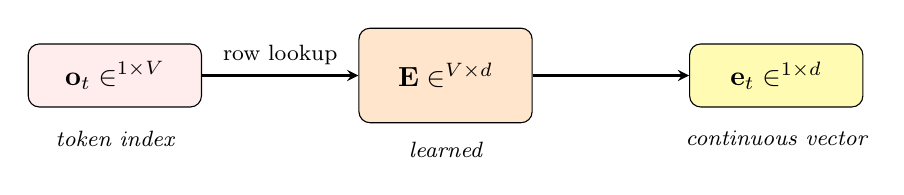
\begin{tikzpicture}[>=stealth]
    \node[draw, rounded corners, fill=pink!30, minimum width=2.2cm, minimum height=0.8cm] (onehot) at (0,0) {$\mathbf{o}_t \in \R^{1 \times V}$};
    \node[draw, rounded corners, fill=orange!20, minimum width=2.2cm, minimum height=1.2cm] (E) at (4.2,0) {$\mathbf{E} \in \R^{V \times d}$};
    \node[draw, rounded corners, fill=yellow!30, minimum width=2.2cm, minimum height=0.8cm] (emb) at (8.4,0) {$\mathbf{e}_t \in \R^{1 \times d}$};
    \draw[->, thick] (onehot) -- (E) node[midway, above, font=\footnotesize] {row lookup};
    \draw[->, thick] (E) -- (emb);
    \node[font=\footnotesize\itshape] at (0,-0.8) {token index};
    \node[font=\footnotesize\itshape] at (4.2,-0.95) {learned};
    \node[font=\footnotesize\itshape] at (8.4,-0.8) {continuous vector};
\end{tikzpicture}
\end{center}

\needspace{0.33\textheight}
\section{Positional Encoding}

The embedding $\mathbf{E}[w_t]$ depends only on the token identity, not on its position $t$ in the sequence. But position matters: ``dog bites man'' and ``man bites dog'' contain the same tokens. We need to inject positional information.

The simplest approach: define a matrix $\mathbf{P} \in \R^{N_{\max} \times d}$ where row $t$ is the positional encoding of position $t$. We \textbf{add} it to the token embedding:
$$\mathbf{x}_t = \mathbf{E}[w_t] + \mathbf{P}[t] \in \R^{1 \times d}$$

The matrix $\mathbf{P}$ can be learned (like $\mathbf{E}$), or it can be fixed. Vaswani et al.\ (2017) used a deterministic sinusoidal encoding:
\begin{align}
\mathbf{P}[t,\, 2k] &= \sin\!\left(\frac{t}{10000^{2k/d}}\right) \\[6pt]
\mathbf{P}[t,\, 2k+1] &= \cos\!\left(\frac{t}{10000^{2k/d}}\right)
\end{align}
for $k = 0, 1, \ldots, d/2 - 1$. Each pair of dimensions oscillates at a different frequency, giving each position a unique signature.

\begin{remark}
The positional encoding is \textbf{added}, not concatenated. Both $\mathbf{E}[w_t]$ and $\mathbf{P}[t]$ have shape $[1 \times d]$, so the sum $\mathbf{x}_t$ also has shape $[1 \times d]$. This preserves the model dimension throughout the architecture.
\end{remark}

For the full sequence:
$$\mathbf{X} = \mathbf{X}_{\text{emb}} + \mathbf{P}_{1:N} \in \R^{N \times d}$$

This is the input to the first transformer block.

\begin{center}
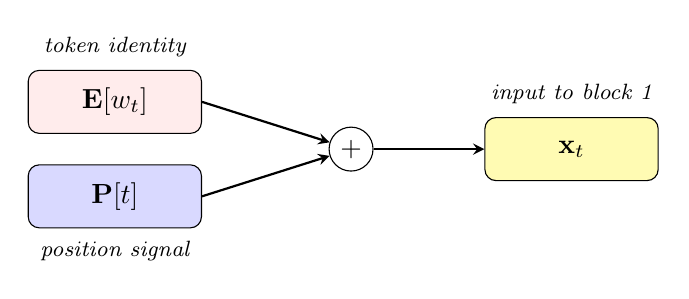
\begin{tikzpicture}[>=stealth]
    \node[draw, rounded corners, fill=pink!30, minimum width=2.2cm, minimum height=0.8cm] (emb) at (0,0.6) {$\mathbf{E}[w_t]$};
    \node[draw, rounded corners, fill=blue!15, minimum width=2.2cm, minimum height=0.8cm] (pos) at (0,-0.6) {$\mathbf{P}[t]$};
    \node[draw, circle, fill=white, inner sep=2pt] (plus) at (3,0) {$+$};
    \node[draw, rounded corners, fill=yellow!30, minimum width=2.2cm, minimum height=0.8cm] (xt) at (5.8,0) {$\mathbf{x}_t$};
    \draw[->, thick] (emb.east) -- (plus);
    \draw[->, thick] (pos.east) -- (plus);
    \draw[->, thick] (plus) -- (xt);
    \node[font=\footnotesize\itshape] at (0,1.3) {token identity};
    \node[font=\footnotesize\itshape] at (0,-1.3) {position signal};
    \node[font=\footnotesize\itshape] at (5.8,0.7) {input to block 1};
\end{tikzpicture}
\end{center}

\needspace{0.33\textheight}
\section{Attention: Motivation}

The next block is \textbf{Masked Multi-Head Attention}. This is the core of the transformer. Before deriving the full mechanism, we motivate it.

Consider the sentence: ``The chicken didn't cross the road because \textbf{it} was too tired.'' The word ``it'' refers to ``chicken''. In ``\ldots because \textbf{it} was too wide'', it refers to ``road''. To compute a useful representation of ``it'', we need to look at the other tokens and determine which ones are relevant.

\textbf{Goal.} Given a token at position $i$ with representation $\mathbf{x}_i \in \R^{1 \times d}$, compute a new representation $\mathbf{a}_i \in \R^{1 \times d}$ that incorporates information from all preceding positions $j \leq i$.

The simplest version: take a weighted sum of the representations of all preceding tokens, where the weights reflect how relevant each token is to position $i$:
$$\mathbf{a}_i = \sum_{j \leq i} \alpha_{ij} \, \mathbf{x}_j, \qquad \alpha_{ij} \geq 0, \qquad \sum_{j \leq i} \alpha_{ij} = 1$$

The constraint $j \leq i$ is the \textbf{causal mask}: token $i$ cannot look at future tokens, since at generation time those tokens have not been produced yet.

How should we compute $\alpha_{ij}$? A natural choice is to use the dot product as a similarity measure, then normalize with a softmax:
$$\alpha_{ij} = \frac{\exp(\mathbf{x}_i \cdot \mathbf{x}_j)}{\sum_{k \leq i} \exp(\mathbf{x}_i \cdot \mathbf{x}_k)}$$

\textbf{Problem.} In this formulation, each $\mathbf{x}_i$ plays three roles simultaneously: the ``query'' (what am I looking for?), the ``key'' (what do I contain?), and the ``value'' (what information do I provide?). Conflating three distinct functions into one vector limits expressiveness.

\needspace{0.33\textheight}
\section{Queries, Keys, and Values}

To separate the three roles, we introduce three learned linear projections.

\begin{definition}[Query, Key, Value]
Given input $\mathbf{x}_i \in \R^{1 \times d}$, define:
\begin{align}
\mathbf{q}_i &= \mathbf{x}_i \, \mathbf{W}^Q \in \R^{1 \times d_k} \\[4pt]
\mathbf{k}_i &= \mathbf{x}_i \, \mathbf{W}^K \in \R^{1 \times d_k} \\[4pt]
\mathbf{v}_i &= \mathbf{x}_i \, \mathbf{W}^V \in \R^{1 \times d_v}
\end{align}
where $\mathbf{W}^Q \in \R^{d \times d_k}$, $\mathbf{W}^K \in \R^{d \times d_k}$, $\mathbf{W}^V \in \R^{d \times d_v}$ are learned weight matrices.
\end{definition}

The \textbf{query} $\mathbf{q}_i$ asks ``what am I looking for?''. The \textbf{key} $\mathbf{k}_j$ answers ``what do I contain?''. The \textbf{value} $\mathbf{v}_j$ is ``what information do I provide if selected?''. Attention scores are computed between queries and keys; values are what gets summed.

\begin{center}
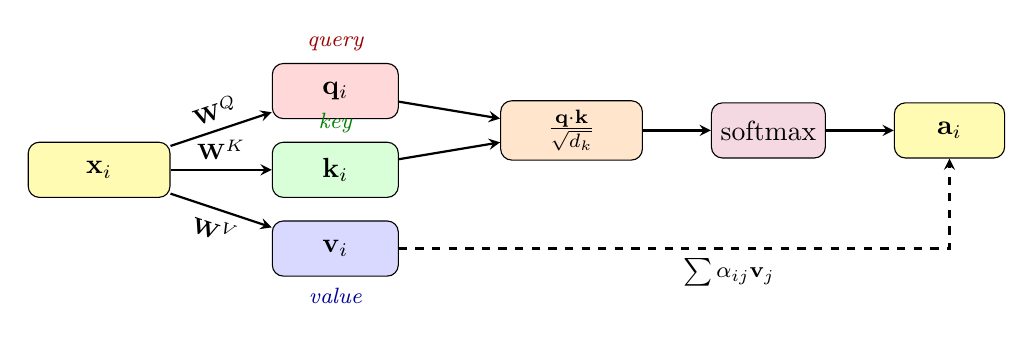
\begin{tikzpicture}[>=stealth]
    \node[draw, rounded corners, fill=yellow!30, minimum width=1.8cm, minimum height=0.7cm] (x) at (0,0) {$\mathbf{x}_i$};
    \node[draw, rounded corners, fill=red!15, minimum width=1.6cm, minimum height=0.7cm] (q) at (3,1) {$\mathbf{q}_i$};
    \node[draw, rounded corners, fill=green!15, minimum width=1.6cm, minimum height=0.7cm] (k) at (3,0) {$\mathbf{k}_i$};
    \node[draw, rounded corners, fill=blue!15, minimum width=1.6cm, minimum height=0.7cm] (v) at (3,-1) {$\mathbf{v}_i$};
    \draw[->, thick] (x) -- (q) node[midway, above, font=\footnotesize, sloped] {$\mathbf{W}^Q$};
    \draw[->, thick] (x) -- (k) node[midway, above, font=\footnotesize] {$\mathbf{W}^K$};
    \draw[->, thick] (x) -- (v) node[midway, below, font=\footnotesize, sloped] {$\mathbf{W}^V$};
    \node[draw, rounded corners, fill=orange!20, minimum width=1.8cm, minimum height=0.7cm] (score) at (6,0.5) {$\frac{\mathbf{q} \cdot \mathbf{k}}{\sqrt{d_k}}$};
    \draw[->, thick] (q) -- (score);
    \draw[->, thick] (k) -- (score);
    \node[draw, rounded corners, fill=purple!15, minimum width=1.4cm, minimum height=0.7cm] (sm) at (8.5,0.5) {softmax};
    \draw[->, thick] (score) -- (sm);
    \node[draw, rounded corners, fill=yellow!30, minimum width=1.4cm, minimum height=0.7cm] (out) at (10.8,0.5) {$\mathbf{a}_i$};
    \draw[->, thick] (sm) -- (out);
    \draw[->, thick, dashed] (v) -- (6,-1) -- (10.8,-1) -- (out);
    \node[font=\footnotesize] at (8,-1.3) {$\sum \alpha_{ij}\mathbf{v}_j$};
    \node[font=\footnotesize\itshape, red!60!black] at (3,1.6) {query};
    \node[font=\footnotesize\itshape, green!50!black] at (3,0.6) {key};
    \node[font=\footnotesize\itshape, blue!60!black] at (3,-1.6) {value};
\end{tikzpicture}
\end{center}

\subsection{Scaled Dot-Product Attention}

The score between positions $i$ and $j$ is:
$$\text{score}(\mathbf{x}_i, \mathbf{x}_j) = \frac{\mathbf{q}_i \cdot \mathbf{k}_j}{\sqrt{d_k}}$$

\begin{proposition}[Scaling preserves unit variance]
If the entries of $\mathbf{q}$ and $\mathbf{k}$ are i.i.d.\ with mean $0$ and variance $1$, then:
$$\E[\mathbf{q}_i \cdot \mathbf{k}_j] = 0, \qquad \Var(\mathbf{q}_i \cdot \mathbf{k}_j) = d_k$$
\end{proposition}

\begin{proof}
The dot product $\mathbf{q}_i \cdot \mathbf{k}_j = \sum_{m=1}^{d_k} q_{im} k_{jm}$ is a sum of $d_k$ independent terms. By independence, $\E[q_{im} k_{jm}] = \E[q_{im}]\E[k_{jm}] = 0$. For the variance:
$$\Var(q_{im} k_{jm}) = \E[q_{im}^2 k_{jm}^2] - (\E[q_{im} k_{jm}])^2 = \E[q_{im}^2]\E[k_{jm}^2] - 0 = 1$$
Summing $d_k$ such terms gives $\Var(\mathbf{q}_i \cdot \mathbf{k}_j) = d_k$.
\end{proof}

So the standard deviation of the raw dot product grows as $\sqrt{d_k}$. For large $d_k$, the dot products become large in magnitude, pushing the softmax into saturation (outputs near 0 or 1) where gradients vanish. Dividing by $\sqrt{d_k}$ normalizes the variance back to 1.

\subsection{Putting It Together}

The attention weight from position $i$ to position $j$ is:
$$\alpha_{ij} = \frac{\exp\!\big(\mathbf{q}_i \cdot \mathbf{k}_j / \sqrt{d_k}\big)}{\sum_{m \leq i} \exp\!\big(\mathbf{q}_i \cdot \mathbf{k}_m / \sqrt{d_k}\big)} \qquad \forall\, j \leq i$$

The attention output is the weighted sum of values:
$$\text{head}_i = \sum_{j \leq i} \alpha_{ij} \, \mathbf{v}_j \in \R^{1 \times d_v}$$

Finally, we apply an output projection $\mathbf{W}^O \in \R^{d_v \times d}$ to map back to the model dimension:
$$\mathbf{a}_i = \text{head}_i \; \mathbf{W}^O \in \R^{1 \times d}$$

\subsection{Shape Summary}

\begin{center}
\renewcommand{\arraystretch}{1.3}
\begin{tabular}{l c}
\hline
\textbf{Object} & \textbf{Shape} \\
\hline
Input $\mathbf{x}_i$ & $[1 \times d]$ \\
$\mathbf{W}^Q, \mathbf{W}^K$ & $[d \times d_k]$ \\
$\mathbf{W}^V$ & $[d \times d_v]$ \\
$\mathbf{q}_i, \mathbf{k}_j$ & $[1 \times d_k]$ \\
$\mathbf{v}_j$ & $[1 \times d_v]$ \\
$\mathbf{q}_i \cdot \mathbf{k}_j$ & scalar \\
$\alpha_{ij}$ & scalar \\
$\text{head}_i$ & $[1 \times d_v]$ \\
$\mathbf{W}^O$ & $[d_v \times d]$ \\
$\mathbf{a}_i$ & $[1 \times d]$ \\
\hline
\end{tabular}
\end{center}

The input and output both have dimension $d$. This is by design: it means attention blocks can be stacked.

\subsection{Parallelization via Matrices}

The computation above describes a single output $\mathbf{a}_i$. For all $N$ positions simultaneously, we pack the embeddings into $\mathbf{X} \in \R^{N \times d}$ and compute:
$$\mathbf{Q} = \mathbf{X}\mathbf{W}^Q, \quad \mathbf{K} = \mathbf{X}\mathbf{W}^K, \quad \mathbf{V} = \mathbf{X}\mathbf{W}^V$$

All $N^2$ pairwise scores are computed in one matrix multiply:
$$\mathbf{S} = \frac{\mathbf{Q}\mathbf{K}^\top}{\sqrt{d_k}} \in \R^{N \times N}$$

The entry $S_{ij}$ is the score from position $i$ to position $j$.

\subsection{The Causal Mask}

The matrix $\mathbf{S}$ contains scores for all pairs $(i,j)$, including $j > i$ (future tokens). To enforce causality, we add a mask matrix $\mathbf{M} \in \R^{N \times N}$:
$$M_{ij} = \begin{cases} 0 & \text{if } j \leq i \\ -\infty & \text{if } j > i \end{cases}$$

Since $e^{-\infty} = 0$, the softmax zeroes out all future positions. The full masked attention is:
$$\text{Attention}(\mathbf{Q}, \mathbf{K}, \mathbf{V}) = \text{softmax}\!\left(\frac{\mathbf{Q}\mathbf{K}^\top}{\sqrt{d_k}} + \mathbf{M}\right) \mathbf{V} \in \R^{N \times d_v}$$

The resulting weight matrix is lower-triangular: position $i$ attends only to positions $1, \ldots, i$.

\begin{center}
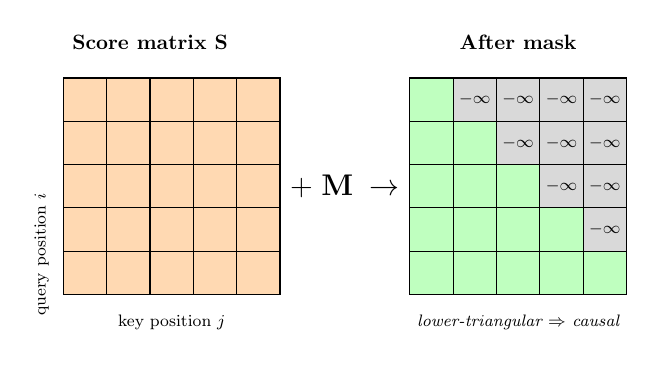
\begin{tikzpicture}[scale=0.55, every node/.style={scale=0.75}]
    % Score matrix (before mask)
    \node[above] at (2,5.5) {\textbf{Score matrix $\mathbf{S}$}};
    \foreach \i in {0,...,4} {
        \foreach \j in {0,...,4} {
            \fill[orange!30] (\j,4-\i) rectangle (\j+1,5-\i);
            \draw (\j,4-\i) rectangle (\j+1,5-\i);
        }
    }
    % Arrow
    \node at (6.5,2.5) {\Large $+\;\mathbf{M}\;\to$};
    % Masked matrix
    \node[above] at (10.5,5.5) {\textbf{After mask}};
    \foreach \i in {0,...,4} {
        \foreach \j in {0,...,4} {
            \pgfmathparse{int(\j<=\i)}
            \ifnum\pgfmathresult=1
                \fill[green!25] (8+\j,4-\i) rectangle (9+\j,5-\i);
                \draw (8+\j,4-\i) rectangle (9+\j,5-\i);
            \else
                \fill[gray!30] (8+\j,4-\i) rectangle (9+\j,5-\i);
                \draw (8+\j,4-\i) rectangle (9+\j,5-\i);
                \node[font=\footnotesize] at (8.5+\j,4.5-\i) {$-\infty$};
            \fi
        }
    }
    % Labels
    \node[below, font=\footnotesize] at (2.5,-0.3) {key position $j$};
    \node[left, font=\footnotesize, rotate=90] at (-0.5,2.5) {query position $i$};
    \node[below, font=\footnotesize\itshape] at (10.5,-0.3) {lower-triangular $\Rightarrow$ causal};
\end{tikzpicture}
\end{center}

\textbf{Computational cost.} The product $\mathbf{Q}\mathbf{K}^\top$ costs $O(N^2 d_k)$. Attention is therefore \textbf{quadratic} in the sequence length $N$.

\needspace{0.33\textheight}
\section{Multi-Head Attention}

A single set of projections $(\mathbf{W}^Q, \mathbf{W}^K, \mathbf{W}^V)$ can learn one type of attention pattern. But tokens relate to each other in many ways: syntactic agreement, coreference, semantic similarity. To capture multiple types of relationships simultaneously, we use \textbf{multiple heads}.

\begin{definition}[Multi-Head Attention]
Given $A$ attention heads, each head $c \in \{1, \ldots, A\}$ has its own weight matrices $\mathbf{W}^{Qc}, \mathbf{W}^{Kc}, \mathbf{W}^{Vc}$. Each head computes:
$$\text{head}^c = \text{Attention}\!\left(\mathbf{X}\mathbf{W}^{Qc},\; \mathbf{X}\mathbf{W}^{Kc},\; \mathbf{X}\mathbf{W}^{Vc}\right) \in \R^{N \times d_v}$$

The heads are concatenated and projected:
$$\text{MultiHead}(\mathbf{X}) = \bigl[\text{head}^1 \;\|\; \text{head}^2 \;\|\; \cdots \;\|\; \text{head}^A\bigr] \, \mathbf{W}^O$$
where $\|$ denotes concatenation along the last axis and $\mathbf{W}^O \in \R^{Ad_v \times d}$.
\end{definition}

\textbf{Shapes.} Each head output is $[N \times d_v]$. Concatenating $A$ heads gives $[N \times Ad_v]$. Multiplying by $\mathbf{W}^O$ gives $[N \times d]$. It is standard to set $d_k = d_v = d/A$ so that $Ad_v = d$ and the total parameter count equals that of a single head with full dimension $d$.

In the original transformer: $d = 512$, $A = 8$, $d_k = d_v = 64$.

\begin{center}
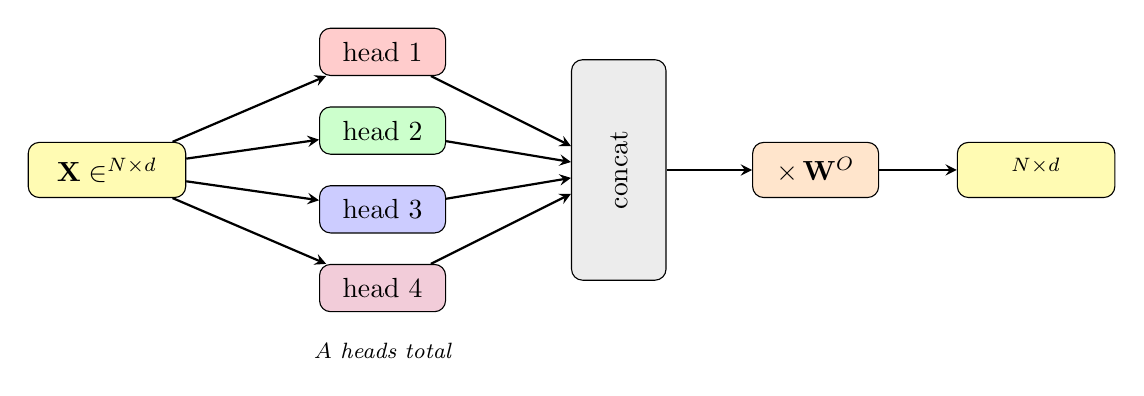
\begin{tikzpicture}[>=stealth]
    \node[draw, rounded corners, fill=yellow!30, minimum width=2cm, minimum height=0.7cm] (X) at (0,0) {$\mathbf{X} \in \R^{N \times d}$};
    \node[draw, rounded corners, fill=red!20, minimum width=1.6cm, minimum height=0.6cm] (h1) at (3.5,1.5) {head 1};
    \node[draw, rounded corners, fill=green!20, minimum width=1.6cm, minimum height=0.6cm] (h2) at (3.5,0.5) {head 2};
    \node[draw, rounded corners, fill=blue!20, minimum width=1.6cm, minimum height=0.6cm] (h3) at (3.5,-0.5) {head 3};
    \node[draw, rounded corners, fill=purple!20, minimum width=1.6cm, minimum height=0.6cm] (h4) at (3.5,-1.5) {head 4};
    \draw[->, thick] (X) -- (h1);  \draw[->, thick] (X) -- (h2);
    \draw[->, thick] (X) -- (h3);  \draw[->, thick] (X) -- (h4);
    \node[draw, rounded corners, fill=gray!15, minimum width=1.2cm, minimum height=2.8cm] (concat) at (6.5,0) {\rotatebox{90}{concat}};
    \draw[->, thick] (h1) -- (concat);  \draw[->, thick] (h2) -- (concat);
    \draw[->, thick] (h3) -- (concat);  \draw[->, thick] (h4) -- (concat);
    \node[draw, rounded corners, fill=orange!20, minimum width=1.6cm, minimum height=0.7cm] (WO) at (9,0) {$\times\,\mathbf{W}^O$};
    \draw[->, thick] (concat) -- (WO);
    \node[draw, rounded corners, fill=yellow!30, minimum width=2cm, minimum height=0.7cm] (out) at (11.8,0) {$\R^{N \times d}$};
    \draw[->, thick] (WO) -- (out);
    \node[font=\footnotesize\itshape] at (3.5,-2.3) {$A$ heads total};
\end{tikzpicture}
\end{center}

\begin{remark}
The multi-head mechanism divides the $d$-dimensional representation into $A$ subspaces of dimension $d/A$ each. Each head learns an independent attention pattern in its subspace. This is strictly more expressive than a single head, because a single head must average over all types of relationships.
\end{remark}

\needspace{0.33\textheight}
\section{Add \& Norm}

The next component (appearing after each sub-layer) is ``Add \& Norm''. This combines two mechanisms: a \textbf{residual connection} and \textbf{layer normalization}.

\subsection{Residual Connections}

Given a sub-layer function $f$ (either attention or feedforward), the residual connection is:
$$\text{output} = f(\mathbf{x}) + \mathbf{x}$$

This creates a direct path for the input to flow through unchanged, while the sub-layer only needs to learn a \textit{correction}. This addresses the vanishing gradient problem: the gradient of $\mathbf{x} + f(\mathbf{x})$ with respect to $\mathbf{x}$ is $\mathbf{I} + \frac{\partial f}{\partial \mathbf{x}}$, which is always at least the identity.

\begin{center}
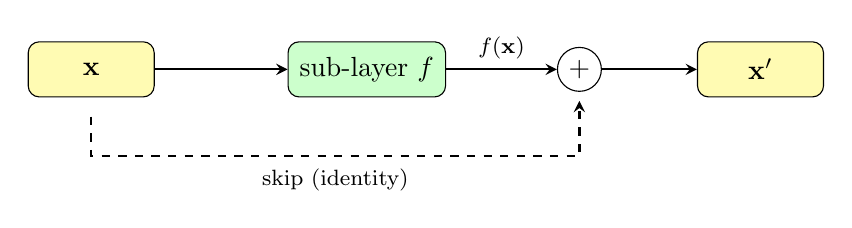
\begin{tikzpicture}[>=stealth]
    \node[draw, rounded corners, fill=yellow!30, minimum width=1.6cm, minimum height=0.7cm] (x) at (0,0) {$\mathbf{x}$};
    \node[draw, rounded corners, fill=green!20, minimum width=2cm, minimum height=0.7cm] (f) at (3.5,0) {sub-layer $f$};
    \node[draw, circle, fill=white, inner sep=2pt] (plus) at (6.2,0) {$+$};
    \node[draw, rounded corners, fill=yellow!30, minimum width=1.6cm, minimum height=0.7cm] (out) at (8.5,0) {$\mathbf{x}'$};
    \draw[->, thick] (x) -- (f);
    \draw[->, thick] (f) -- (plus) node[midway, above, font=\footnotesize] {$f(\mathbf{x})$};
    \draw[->, thick] (plus) -- (out);
    \draw[->, thick, dashed] (0,-0.6) -- (0,-1.1) -- (6.2,-1.1) -- (6.2,-0.4);
    \node[font=\footnotesize] at (3.1,-1.4) {skip (identity)};
\end{tikzpicture}
\end{center}

\subsection{Layer Normalization}

Given a vector $\mathbf{x} \in \R^d$, layer normalization (Ba et al., 2016) normalizes it to zero mean and unit variance, then applies a learned affine transformation.

\textbf{Step 1.} Compute the mean and standard deviation over the $d$ components of $\mathbf{x}$:
\begin{align}
\mu &= \frac{1}{d} \sum_{i=1}^{d} x_i \\[6pt]
\sigma &= \sqrt{\frac{1}{d} \sum_{i=1}^{d} (x_i - \mu)^2}
\end{align}

\textbf{Step 2.} Normalize and apply learned parameters $\gamma, \beta \in \R^d$:
$$\text{LayerNorm}(\mathbf{x}) = \gamma \odot \frac{\mathbf{x} - \mu}{\sigma + \epsilon} + \beta$$

where $\odot$ is element-wise multiplication and $\epsilon > 0$ is a small constant for numerical stability. The parameters $\gamma$ (gain) and $\beta$ (offset) are learned during training.

\begin{remark}
Layer normalization is applied to a \textbf{single token's vector}, not across the batch or across positions. It is the $z$-score from statistics, applied dimension-wise to one embedding.
\end{remark}

\subsection{Order of Operations}

In the original transformer (Vaswani et al., 2017), the order is sub-layer $\to$ add $\to$ norm (``post-norm''). Most modern implementations use the ``pre-norm'' variant: norm $\to$ sub-layer $\to$ add. We write the pre-norm version, since it is now standard:
\begin{align}
\mathbf{z} &= \text{LayerNorm}(\mathbf{x}) \\
\mathbf{x}' &= f(\mathbf{z}) + \mathbf{x}
\end{align}

\needspace{0.33\textheight}
\section{Feed-Forward Network}

After the first Add \& Norm, the diagram shows a \textbf{Feed Forward} block. This is a standard two-layer fully connected network, applied independently and identically to each token position:
$$\text{FFN}(\mathbf{x}) = \text{ReLU}(\mathbf{x}\,\mathbf{W}_1 + \mathbf{b}_1)\,\mathbf{W}_2 + \mathbf{b}_2$$

where $\mathbf{W}_1 \in \R^{d \times d_{\text{ff}}}$, $\mathbf{W}_2 \in \R^{d_{\text{ff}} \times d}$, and $\text{ReLU}(z) = \max(0, z)$.

The hidden dimension $d_{\text{ff}}$ is typically $4d$. In the original transformer, $d = 512$ and $d_{\text{ff}} = 2048$.

\begin{center}
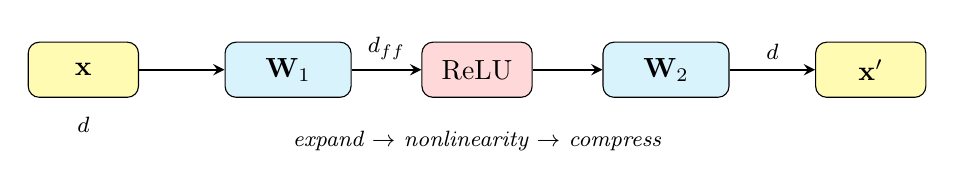
\begin{tikzpicture}[>=stealth]
    \node[draw, rounded corners, fill=yellow!30, minimum width=1.4cm, minimum height=0.7cm] (x) at (0,0) {$\mathbf{x}$};
    \node[draw, rounded corners, fill=cyan!15, minimum width=1.6cm, minimum height=0.7cm] (W1) at (2.6,0) {$\mathbf{W}_1$};
    \node[draw, rounded corners, fill=red!15, minimum width=1.4cm, minimum height=0.7cm] (relu) at (5,0) {ReLU};
    \node[draw, rounded corners, fill=cyan!15, minimum width=1.6cm, minimum height=0.7cm] (W2) at (7.4,0) {$\mathbf{W}_2$};
    \node[draw, rounded corners, fill=yellow!30, minimum width=1.4cm, minimum height=0.7cm] (out) at (10,0) {$\mathbf{x}'$};
    \draw[->, thick] (x) -- (W1);
    \draw[->, thick] (W1) -- (relu) node[midway, above, font=\footnotesize] {$d_{\text{ff}}$};
    \draw[->, thick] (relu) -- (W2);
    \draw[->, thick] (W2) -- (out) node[midway, above, font=\footnotesize] {$d$};
    \node[font=\footnotesize] at (0,-0.7) {$d$};
    \node[font=\footnotesize\itshape] at (5,-0.9) {expand $\to$ nonlinearity $\to$ compress};
\end{tikzpicture}
\end{center}

\textbf{Key point.} The FFN processes each position independently: it sees only the $d$-dimensional vector at one position, with no interaction between positions. The attention layer is the only component that mixes information across positions.

After the FFN, there is another Add \& Norm (the second one in each block).

\needspace{0.33\textheight}
\section{Stacking: $L$ Blocks}

The block (Masked Multi-Head Attention $\to$ Add \& Norm $\to$ Feed Forward $\to$ Add \& Norm) is repeated $L$ times. In pre-norm convention, one block computes:
\begin{align}
\mathbf{O} &= \mathbf{X} + \text{MultiHead}\!\left(\text{LayerNorm}(\mathbf{X})\right) \\[4pt]
\mathbf{H} &= \mathbf{O} + \text{FFN}\!\left(\text{LayerNorm}(\mathbf{O})\right)
\end{align}

The output $\mathbf{H} \in \R^{N \times d}$ has the same shape as the input $\mathbf{X} \in \R^{N \times d}$. This is what makes stacking possible: the output of block $\ell$ is the input to block $\ell + 1$.

\begin{center}
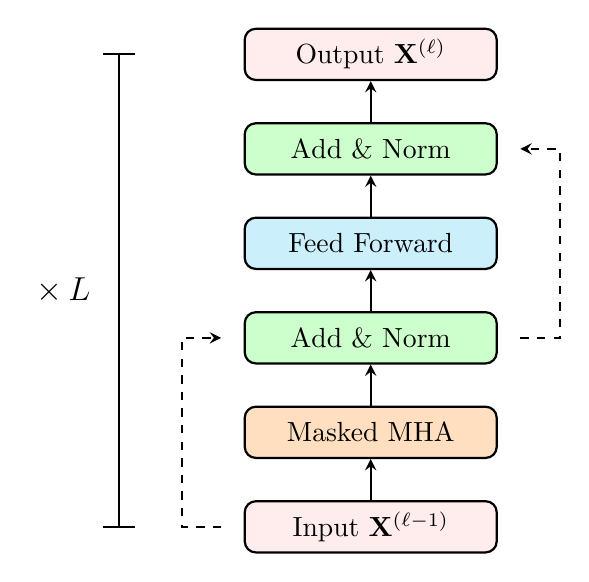
\begin{tikzpicture}[>=stealth,
    block/.style={draw, rounded corners, minimum width=3.2cm, minimum height=0.65cm, thick}]
    \node[block, fill=pink!30] (input) at (0,0) {Input $\mathbf{X}^{(\ell-1)}$};
    \node[block, fill=orange!25] (mha) at (0,1.2) {Masked MHA};
    \node[block, fill=green!20] (an1) at (0,2.4) {Add \& Norm};
    \node[block, fill=cyan!20] (ffn) at (0,3.6) {Feed Forward};
    \node[block, fill=green!20] (an2) at (0,4.8) {Add \& Norm};
    \node[block, fill=pink!30] (output) at (0,6.0) {Output $\mathbf{X}^{(\ell)}$};
    \draw[->, thick] (input) -- (mha);
    \draw[->, thick] (mha) -- (an1);
    \draw[->, thick] (an1) -- (ffn);
    \draw[->, thick] (ffn) -- (an2);
    \draw[->, thick] (an2) -- (output);
    \draw[->, thick, dashed] (-1.9,0) -- (-2.4,0) -- (-2.4,2.4) -- (-1.9,2.4);
    \draw[->, thick, dashed] (1.9,2.4) -- (2.4,2.4) -- (2.4,4.8) -- (1.9,4.8);
    \draw[thick] (-3.2,0) -- (-3.2,6.0);
    \draw[thick] (-3.4,0) -- (-3.0,0);
    \draw[thick] (-3.4,6.0) -- (-3.0,6.0);
    \node[font=\large] at (-3.9,3.0) {$\times\, L$};
\end{tikzpicture}
\end{center}

Typical depth: $L = 12$ for small models (GPT-2), $L = 96$ for large models (GPT-3), $L = 126$ for Llama 3.1 405B.

At the very top of the final block there is one additional LayerNorm applied to $\mathbf{X}^{(L)}$ before passing to the output stage.

\needspace{0.33\textheight}
\section{Linear + Softmax (The Output Head)}

The output of the last transformer block, after the final LayerNorm, is a matrix $\mathbf{H} \in \R^{N \times d}$. We take the row corresponding to the last token, $\mathbf{h}_N \in \R^{1 \times d}$, and map it to a probability distribution over the vocabulary $\mathcal{V}$.

\subsection{The Linear Layer (Unembedding)}

We need to go from $\R^d \to \R^V$. A natural choice: reuse the embedding matrix $\mathbf{E} \in \R^{V \times d}$ from \S2, transposed. This is called \textbf{weight tying}.

The \textbf{logit} (unnormalized score) for each token $k \in \mathcal{V}$ is:
$$u_k = \mathbf{h}_N \cdot \mathbf{E}[k]$$

In matrix form:
$$\mathbf{u} = \mathbf{h}_N \, \mathbf{E}^\top \in \R^{1 \times V}$$

The score for token $k$ is the dot product between the contextual representation $\mathbf{h}_N$ and the embedding of token $k$. Tokens whose embeddings are ``close'' to $\mathbf{h}_N$ receive high scores.

\begin{center}
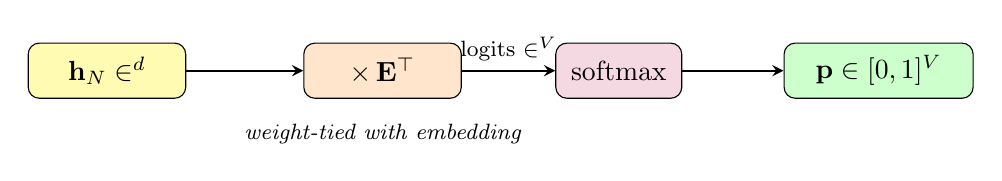
\begin{tikzpicture}[>=stealth]
    \node[draw, rounded corners, fill=yellow!30, minimum width=2cm, minimum height=0.7cm] (h) at (0,0) {$\mathbf{h}_N \in \R^d$};
    \node[draw, rounded corners, fill=orange!20, minimum width=2cm, minimum height=0.7cm] (linear) at (3.5,0) {$\times\,\mathbf{E}^\top$};
    \node[draw, rounded corners, fill=purple!15, minimum width=1.6cm, minimum height=0.7cm] (sm) at (6.5,0) {softmax};
    \node[draw, rounded corners, fill=green!20, minimum width=2.4cm, minimum height=0.7cm] (p) at (9.8,0) {$\mathbf{p} \in [0,1]^V$};
    \draw[->, thick] (h) -- (linear);
    \draw[->, thick] (linear) -- (sm) node[midway, above, font=\footnotesize] {logits $\in \R^V$};
    \draw[->, thick] (sm) -- (p);
    \node[font=\footnotesize\itshape] at (3.5,-0.8) {weight-tied with embedding};
\end{tikzpicture}
\end{center}

\begin{remark}
Weight tying means $\mathbf{E}$ must simultaneously be a good input representation (mapping tokens to $\R^d$) and a good output projection (mapping $\R^d$ back to token scores). This halves the number of vocabulary-related parameters and serves as a regularizer.
\end{remark}

\subsection{Softmax}

The logits $\mathbf{u} \in \R^{1 \times V}$ are real-valued and unnormalized. We convert them to a probability distribution using the softmax function:
$$p(w_{N+1} = k \mid w_{1:N}) = \frac{\exp(u_k)}{\sum_{j=1}^{V} \exp(u_j)}$$

This satisfies $p_k > 0$ for all $k$ and $\sum_k p_k = 1$.

\textbf{Numerical stability.} In practice we compute $\text{softmax}(\mathbf{u} - \max_k u_k)$. Subtracting the maximum does not change the output (the constant cancels in numerator and denominator) but prevents overflow in the exponential.

\needspace{0.33\textheight}
\section{Training}

The model is trained by \textbf{maximum likelihood}, which is equivalent to minimizing the \textbf{cross-entropy loss}.

At position $t$, the model outputs a distribution $\hat{p}(\cdot \mid w_{1:t})$ over $\mathcal{V}$. The true next token is $w_{t+1}$, which defines a one-hot distribution. The cross-entropy between them is:
$$\mathcal{L}_t = -\log \hat{p}(w_{t+1} \mid w_{1:t})$$

For a sequence of $T$ tokens, we average:
$$\mathcal{L} = -\frac{1}{T} \sum_{t=1}^{T} \log \hat{p}(w_{t+1} \mid w_{1:t})$$

This is minimized via gradient descent (typically Adam) with backpropagation through all $L$ transformer blocks.

\textbf{Key advantage over RNNs.} Thanks to the causal mask, the loss at every position $t$ can be computed \textbf{in parallel} during training. The entire sequence is processed in a single forward pass. This is why transformers are faster to train than recurrent models, despite having quadratic attention cost.

\needspace{0.33\textheight}
\section{Generation (Inference)}

Given a trained model and a prompt $w_{1:N}$, we generate text by repeated next-token prediction:

\begin{enumerate}
\item Set $t \gets N$.
\item \textbf{Repeat:}
\begin{enumerate}
    \item Compute $\mathbf{h}_t^{(L)} = f_\Theta(w_{1:t})$ \hfill (forward pass)
    \item $\mathbf{u} \gets \mathbf{h}_t^{(L)} \, \mathbf{E}^\top$ \hfill (logits)
    \item $\mathbf{p} \gets \text{softmax}(\mathbf{u})$ \hfill (probabilities)
    \item $w_{t+1} \sim \text{Sample}(\mathbf{p})$ \hfill (choose next token)
    \item $t \gets t + 1$
\end{enumerate}
\item \textbf{Until} end-of-sequence token or max length.
\item \textbf{Return} $w_{N+1:t}$.
\end{enumerate}

The sampling strategy in step 2(d) controls the quality/diversity tradeoff:

\textbf{Greedy decoding:} Always take $w_{t+1} = \arg\max_k p_k$. Deterministic, but repetitive.

\textbf{Top-$k$ sampling:} Zero out all but the $k$ most probable tokens, renormalize, and sample. When $k = 1$, this reduces to greedy decoding.

\textbf{Top-$p$ (nucleus) sampling:} Retain the smallest set $\mathcal{S}$ such that $\sum_{w \in \mathcal{S}} p(w) \geq p$, renormalize, and sample. This adapts the number of candidates to the shape of the distribution.

\needspace{0.33\textheight}
\section{Parameter Count and Scaling}

\begin{proposition}[Parameter count per block]
The number of non-embedding parameters per transformer block is $12\,d^2$ (assuming $d_{\text{ff}} = 4d$ and $d_k = d_v = d/A$).
\end{proposition}

\begin{proof}
The attention sub-layer has four weight matrices:
$$\underbrace{\mathbf{W}^Q, \mathbf{W}^K, \mathbf{W}^V}_{\text{each } d \times d_k \text{ per head}} \text{ and } \mathbf{W}^O$$
With $A$ heads and $d_k = d/A$, each of $\mathbf{W}^Q, \mathbf{W}^K, \mathbf{W}^V$ contributes $A \cdot d \cdot (d/A) = d^2$ parameters, and $\mathbf{W}^O \in \R^{d \times d}$ contributes $d^2$. Total for attention: $4d^2$.

The FFN has $\mathbf{W}_1 \in \R^{d \times 4d}$ and $\mathbf{W}_2 \in \R^{4d \times d}$, contributing $4d^2 + 4d^2 = 8d^2$.

Total per block: $4d^2 + 8d^2 = 12d^2$.
\end{proof}

For $L$ blocks, the total non-embedding parameter count is:
$$N_{\text{params}} \approx 12\, L\, d^2$$

\textbf{Example.} GPT-3: $L = 96$, $d = 12{,}288$. Then $12 \times 96 \times 12{,}288^2 \approx 175$ billion parameters.

Kaplan et al.\ (2020) showed that the loss follows a \textbf{power law} in model size $N$, dataset size $D$, and compute $C$:
\begin{align}
\mathcal{L}(N) &\propto N^{-\alpha_N} \\[4pt]
\mathcal{L}(D) &\propto D^{-\alpha_D} \\[4pt]
\mathcal{L}(C) &\propto C^{-\alpha_C}
\end{align}

These \textbf{scaling laws} allow us to predict the performance of larger models from small-scale experiments.

\needspace{0.33\textheight}
\section{Summary: Complete Forward Pass}

Collecting everything, the forward pass of a decoder-only transformer language model is:

\begin{enumerate}
\item \textit{Embed + Position} (\S2--3):
$$\mathbf{x}_t = \mathbf{E}[w_t] + \mathbf{P}[t], \qquad \mathbf{X}^{(0)} = [\mathbf{x}_1; \ldots; \mathbf{x}_N] \in \R^{N \times d}$$

\item \textit{Transformer Blocks} (\S4--9), for $\ell = 1, \ldots, L$:
\begin{align}
\mathbf{O}^{(\ell)} &= \mathbf{X}^{(\ell-1)} + \text{MHA}\!\left(\text{LN}\!\left(\mathbf{X}^{(\ell-1)}\right)\right) \\[4pt]
\mathbf{X}^{(\ell)} &= \mathbf{O}^{(\ell)} + \text{FFN}\!\left(\text{LN}\!\left(\mathbf{O}^{(\ell)}\right)\right)
\end{align}

\item \textit{Final LayerNorm}: $\mathbf{H} = \text{LayerNorm}(\mathbf{X}^{(L)})$

\item \textit{Output Head} (\S10):
$$\mathbf{u} = \mathbf{H}[N]\; \mathbf{E}^\top \in \R^{1 \times V}, \qquad \mathbf{p} = \text{softmax}(\mathbf{u})$$
\end{enumerate}

\end{document}
